% Results. Numbers are carried from artifacts/eval/exp1b/tables.md, artifacts/eval/exp2/tables.md and the findings
% named in each comment; tables are generated by paper/tables/make_tables.py, the figure by
% paper/figures/success_by_level.py. \TBD marks results not yet collected.
\providecommand{\TBD}[1]{\textcolor{red}{[TBD: #1]}}

\section{Results}
\label{sec:results}

\subsection{Autonomous mission generalization}
\label{sec:results-exp1}

The frozen baselines match the proposed runtime wherever their models cover the situation, and stop wherever they do
not. On the seven covered instances every method succeeded in every run (7/7 each, Fig.~\ref{fig:success-level}). On
the six held-out instances the proposed runtime succeeded in all 18 runs, a Wilson 95\% interval from 0.82 to 1.00.
PLEXIL and EUROPA\,$\rightarrow$\,PLEXIL succeeded in none of their six runs each, an interval from 0 to 0.39. The
drop is a step at L2, the first level at which the frozen model lacks a relation, and the curve of the proposed
runtime stays flat through L4.
% Wilson intervals: evaluation.tables.wilson_ci(18, 18) = (0.82, 1.00); wilson_ci(0, 6) = (0, 0.39).

The baselines did not fail by acting wrongly. Every held-out baseline run detected the anomaly through the goal
checks its covered brief asks for, repeated the failing call up to its retry budget, asked mission control for a new
procedure and held in a safe state. The boundary they met is the coverage of their frozen models, which is the
boundary H1 predicts. A larger retry budget would not have moved it: offline reruns of both baselines on every
held-out state with one, two, three and five attempts per call always ended in the same escalation, and only the
number of repeats before it changed (Section~\ref{sec:setup-baselines}).
% F136, F143: 48 offline runs, outcome "detected -> escalated" at every N.

The sharpest case is L3. Every piece of its solution exists in both baselines' libraries: Mission A's reset and
Mission B's pick, carry and place. Only the composition is missing, and neither baseline could form it. The proposed
runtime formed it in all six L3 runs. It read the module fault from the unit's telemetry, took the failed module out of
the bay, fetched the spare and reset the unit. The same held-out runs took more reasoning steps than covered ones, a
median of 50 against 23.
% step_count medians over artifacts/eval/exp1b/rows (Ours held_out 50.0, covered 23).

\begin{figure}[t]
  \centering
  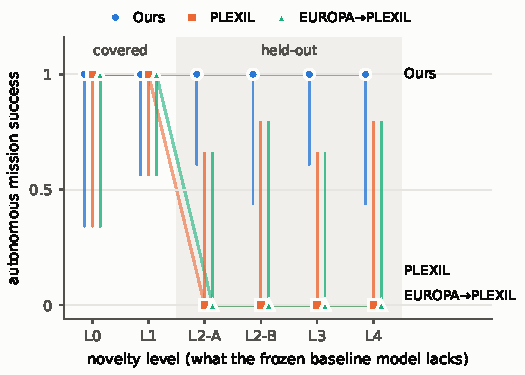
\includegraphics[width=\columnwidth]{figures/success_by_level.pdf}
  \caption{Autonomous mission success of the three methods at each novelty level of Experiment I, with Wilson 95\%
  intervals. Runs per level: Ours 2, 5, 6, 3, 6, 3; each baseline 2, 5, 2, 1, 2, 1.}
  \label{fig:success-level}
\end{figure}

\subsection{Human independence}
\label{sec:results-alfus}

On the held-out instances the methods also separate on every ALFUS measure of human independence
(Table~\ref{tab:independence}). Each held-out baseline run ended in one new-procedure request, so all twelve required
ground re-authoring, and in each of them the highest interaction level was the assignment of a mission task. The
baselines' robots then waited. The median fraction of held-out mission time spent idle for the ground was 0.634 for
PLEXIL and 0.499 for EUROPA\,$\rightarrow$\,PLEXIL, against 0.026 for the proposed runtime. The proposed runtime sent no
new-procedure request in its 18 held-out runs. Its ten requests were three authorizations, all for the L4 donor removal
and all granted, and seven information requests, which mission control answered with no data beyond the robot's own
queries. Its highest interaction level was a tactical goal, the approval of one held call, in each of the three L4
runs, and none in the other 15.
% artifacts/eval/exp1b/tables.md, interaction table (evaluation/tables.py interaction_table; preregistration §4:
% medians with percentile bootstrap 95% intervals over runs, level as the distribution over runs). Idle, held-out:
% PLEXIL 0.634 [0.475, 0.716], EUROPA 0.499 [0.320, 0.630], Ours 0.026 [0.000, 0.162]. Highest level per run,
% held-out: mission_task 6 (each baseline); Ours none 15, tactical_goal 3. The previous draft's 0.608 and 0.483 were
% means over runs.

The proposed runtime also needed less of mission control's time and ran longer without it. Its median human
intervention ratio on held-out runs is 0.080, with an interval from 0.000 to 0.240, against 0.617 for PLEXIL and 0.485
for EUROPA\,$\rightarrow$\,PLEXIL. Its median longest autonomous stretch is 1029\,s against 179\,s and 319\,s. Each
interval is a percentile bootstrap 95\% interval over runs, six per baseline and 18 for the proposed runtime. For the
ratio, the idle fraction and the stretch alike, the interval of the proposed runtime does not overlap either
baseline's. Half of its held-out runs sent no request and have a ratio of zero. The ratio of the other half is above
zero because every request costs a fixed 300\,s of mission control's decision time (Section~\ref{sec:setup-operator}).
The ratio scales linearly with that assumption, while the request counts and the re-authoring flag do not depend on
it.
% artifacts/eval/exp1b/tables.md, interaction table, held-out: HIR Ours 0.080 [0.000, 0.240], PLEXIL 0.617
% [0.461, 0.696], EUROPA 0.485 [0.313, 0.613]; stretch (s) Ours 1029 [770, 1096], PLEXIL 179 [122, 353], EUROPA 319
% [182, 668]. No overlap: HIR 0.240 < 0.313, idle 0.162 < 0.320, stretch 770 > 668. Nine of the 18 held-out Ours runs
% sent no request (requests_* 0, HIR 0 in artifacts/eval/exp1b/rows). The previous draft's 0.136, 0.591, 0.470, 955 s,
% 218 s and 390 s were means over runs.

Autonomy costs mission time. On covered instances the proposed runtime took a median 538\,s against 264\,s for PLEXIL
and 265\,s for EUROPA\,$\rightarrow$\,PLEXIL. Every capability call waits for a reasoning step, and the model also
chose extra work, such as inspecting the site again after the objective was verified. Mission time understates the
cost of that reasoning, and so overstates the human intervention ratio of the proposed runtime, which divides by
mission time. A reasoning call took a median 19.9\,s of wall clock (interquartile range from 11.3 to 38.7\,s), and the
simulation advanced 0.237\,s of mission time per wall-clock second during the calls. Counted in full, the latency
raises the covered median mission time of the proposed runtime from 538\,s to 825\,s, an upper bound on the cost of
reasoning for a model served at this latency.
% medians of mission_elapsed_s over artifacts/eval/exp1b/rows, covered: 538.0, 263.7, 265.2.
% artifacts/eval/exp1b/reasoning_latency.md (experiments/analysis/reasoning_latency.py), all 25 Ours runs: per-call
% wall latency 19.9 [IQR 11.3, 38.7] s; 0.237 mission s per wall s in calls (pooled); covered medians: recorded 538,
% latency in full 825 (= mission_elapsed_s - mission time in calls + wall time in calls, per run). Upper bound: the
% runtime keeps reasoning while a request is open, and those calls would overlap mission control's decision time; with
% no request open the figure is exact for this latency. Held-out median HIR with the latency in full: 0.036 (recorded
% 0.080).

\begin{table*}[t]
  \centering
  \caption{Human independence in Experiment I (NIST ALFUS). HIR: human intervention ratio. Requests: authorization /
  new procedure / information. Highest level: runs by the most human-directed ALFUS level mission control acted at
  (none: no answer directed the robot). Re-authoring: runs that needed a new procedure from the ground. Idle: fraction
  of mission time waiting on the ground. Stretch: longest autonomous stretch. HIR, idle and stretch: median over runs
  [percentile bootstrap 95\% interval].}
  \label{tab:independence}
  \small
  \resizebox{\textwidth}{!}{\begin{tabular}{llrrcccrr}
\toprule
method & coverage & success & HIR & requests A / N / I & highest level & re-authoring & idle & stretch (s) \\
\midrule
Ours & covered & 7/7 & 0.073 & 0 / 0 / 1 & none & 0 & 0.025 & 504 \\
 & held-out & 18/18 & 0.136 & 3 / 0 / 7 & tactical goal & 0 & 0.085 & 955 \\
PLEXIL & covered & 7/7 & 0.000 & 0 / 0 / 0 & none & 0 & 0.000 & 329 \\
 & held-out & 0/6 & 0.591 & 0 / 6 / 0 & mission task & 6 & 0.608 & 218 \\
EUROPA\,$\rightarrow$\,PLEXIL & covered & 7/7 & 0.000 & 0 / 0 / 0 & none & 0 & 0.000 & 325 \\
 & held-out & 0/6 & 0.470 & 0 / 6 / 0 & mission task & 6 & 0.483 & 390 \\
\bottomrule
\end{tabular}
}
\end{table*}

\subsection{Trustworthiness of open reasoning}
\label{sec:results-trust}

Open reasoning did not buy its success by crossing boundaries. No method declared a completion that the external
evaluator did not confirm, in 51 scored runs. The guard of the proposed runtime held three proposals, all donor
removals from an energized unit in L4, and none executed before mission control granted it. The evaluator, which reads
simulator truth for every method alike, counted no removal without approval, no dropped item and no execution during a
latched fault (Table~\ref{tab:violations}). It counted seven unintended contacts for the proposed runtime. Six fell in
one L3 run, in 0.6\,s of docking beside the unit's cradle while the rover carried the removed battery module. The
baselines' failed place attempts on the occupied stand pushed the occupying container by 5.9\,cm three times.
% F142: 6 windows in ours_l3_bess_r2 (0.6 s), 1 in covered B battery delivery (20 ms); collateral PLEXIL 1, EUROPA 2.

Every capability call of the proposed runtime carries its proposal, guard outcome, execution result and verification
in the trace (451 of 451). Every PLEXIL call at the capability boundary joins to the plan node that issued it (81 of
81). A ground team can therefore reconstruct what each method knew and did at each step, the requirement that
Section~\ref{sec:requirements} derives from lunar operations.

These counts show that the boundaries held in the runs that happened. They do not show which component held them,
because the components rarely acted in these runs. The guard fired only in L4, and the verifier never had to catch a
physical failure, since none occurred. Section~\ref{sec:results-ablation} removes each component in turn against
injected faults.

\begin{table}[t]
  \centering
  \caption{Constraint violations counted by the external evaluator from simulator truth, identically for every method.}
  \label{tab:violations}
  \small
  \resizebox{\columnwidth}{!}{\begin{tabular}{llrrrrrr}
\toprule
method & coverage & runs & unintended contact & dropped item & collateral change & execution in fault & removal w/o approval \\
\midrule
Ours & covered & 7 & 1 & 0 & 0 & 0 & 0 \\
 & held-out & 18 & 6 & 0 & 0 & 0 & 0 \\
PLEXIL & covered & 7 & 0 & 0 & 0 & 0 & 0 \\
 & held-out & 6 & 0 & 0 & 1 & 0 & 0 \\
EUROPA\,$\rightarrow$\,PLEXIL & covered & 7 & 0 & 0 & 0 & 0 & 0 \\
 & held-out & 6 & 0 & 0 & 2 & 0 & 0 \\
\bottomrule
\end{tabular}
}
\end{table}

\subsection{Cost of extending the mission envelope}
\label{sec:results-exp2}

Adding a capability after the freeze took the three methods similar time and very different kinds of change
(Table~\ref{tab:extension}). Each extension engineer, a fresh Claude session given only the extension specification
and the validation suite, passed the suite on its first validation run. Active time was 54.5, 46.3 and 53.4 minutes.
Waiting on the simulation dominated all three, and the work outside that wait took 4.7 minutes for the proposed
runtime, 10.8 for PLEXIL and 20.8 for EUROPA\,$\rightarrow$\,PLEXIL.

The kind of change is the sharper result. The proposed runtime registered the capability contract and made a scan
reading a verified fact the model sees. It added no rule about when to scan or what to do when a record is wrong.
PLEXIL's engineer wrote that knowledge as a procedure: check the named serial at the recorded source, then the other
supports of the same kind, then all 13 staging supports in a fixed order, else ask mission control and hold.
EUROPA's engineer modelled item identity as state with a sensing activity, and narrowed the candidate supports in the
host's fact translation. Line counts are not comparable across Python, PLEXIL and NDDL, and the table reports them
only as the size of each change.

On the hidden cases each method went from failing both before its extension to full success after it: 6 of 6 runs for
the proposed runtime and 2 of 2 for each baseline. Before the extension, all three methods delivered the unit that the
inventory record pointed to, which was the wrong unit. The baselines ended their plans normally. The proposed runtime
reported both deliveries as complete, two false completions, because its verifier could confirm a placement but not an
identity. Once the scanner made identity observable, the same verifier turned each reading into a fact, and no false
completion recurred.

The proposed runtime searched less systematically than PLEXIL's fixed sweep. It needed from 12 to 17 scans to find the
mislocated unit, where PLEXIL needed 6 and EUROPA\,$\rightarrow$\,PLEXIL 3. One engineer per method, and a coding
assistant in that role, limit what these times can claim (Section~\ref{sec:limitations}).
% exp2 tables.md section 3: post_ours_h1 scans 17, 12 (after F147), 15; post_plexil_h1 6; post_europa_h1_f145 3.

\begin{table*}[t]
  \centering
  \caption{Experiment II: engineering effort to reach the validation suite, and success on the hidden cases before and
  after the extension. Mission artifacts: prompts, contracts and runtime (Ours), plans (PLEXIL), domain and host
  (EUROPA\,$\rightarrow$\,PLEXIL). Supporting files: adapter, offline tests and documentation.}
  \label{tab:extension}
  \small
  \begin{tabular}{lrrrrrrrr}
\toprule
method & active (min) & waiting on validation (min) & other work (min) & validation runs & mission artifacts (+/$-$) & supporting files (+/$-$) & held-out before & held-out after \\
\midrule
Ours & 54.5 & 49.8 & 4.7 & 1 & +49/-3 & +0/-0 & 0/2 & 6/6 \\
PLEXIL & 46.3 & 35.4 & 10.8 & 1 & +89/-5 & +122/-3 & 0/2 & 2/2 \\
EUROPA\,$\rightarrow$\,PLEXIL & 53.4 & 32.5 & 20.8 & 1 & +144/-27 & +53/-0 & 0/2 & 2/2 \\
\bottomrule
\end{tabular}

\end{table*}

\subsection{Re-authoring cost of the held-out cases}
\label{sec:results-reauthoring}

\TBD{per baseline and held-out case: active engineering time, plan nodes or domain elements added, validation runs;
the proposed runtime needed none (0 of 18 held-out runs re-authored).}

\subsection{Ablations of the harness}
\label{sec:results-ablation}

\TBD{offline counterfactual decisions per accident and variant (F148 rubric) and the live consequences.}
